\subsection{Software}
Softwareseitig haben wir Octave benutzt. Als freie Alternative zu Matlab vereint Octave gute Performance, syntaktische Gleichheit zu Matlab, sowie kostenfreie Benutzung unter einem Dach. Im Vergleich mit Python haben wir festgestellt, dass die Geschwindigkeit aufwendiger Rechnungen, wie der Korrelation, bei Python schlechter ist. Somit haben wir uns für Ocatve entschieden. Um unseres selbstgeschriebenes Programm zu verifizieren haben wir eine Autokorrelation durchgeführt und diese mit der von Audactity berechneten AKF verglichen. Wir sind dabei zu dem Ergebnis gekommen, dass unser Programm funktioniert. Zur Aufnahme der Audiosignale haben wir ebenfalls die Software Audacity benutzt.
\subsection{Hardware}
Uns standen zwei hochwertige Kondensatormikrofone (M5 Matched Pair Compac 1/2" Cardioid Condenser Microphones von Rode) zur Verfügung. Diese Mikrofone sind für dieses Projekt besonders geeignet, da durch die Abstimmung (matched pair) nur die Unterschiede im Signal vor der Aufnahme Einfluss auf die Korrelation haben. Da es sich um Mikrofone mit Nierencharakteristik handelt, ist jedoch zu beachten, dass es sich bei den Aufnahmen um Gerichtete handelt und nicht wie bei Mikrofonen mit Kugelcharakteristik von einer Abbildung des gesamten gemessenen Raumes ausgegangen werden kann. Für die Digitalisierung der Signale stand uns ein hochwertiges Audio-USB-Interface (Scarlett 2i2 von Focusrite) zur Verfügung. Die Aufnahmen wurden in .wav gespeichert und sind somit verlustfrei. Außerdem konnten wir ein Stativ mit einer Mikrofonschiene verwenden, wodurch die Mikrofone konstanten Abstand hatten. Zur Erzeugung eines reproduzierbaren Klangsignales wurde eine portable Bluetooth-Anlage (Soundlink III von Bose) verwendet.

\begin{figure}[ht!]
  \centering
  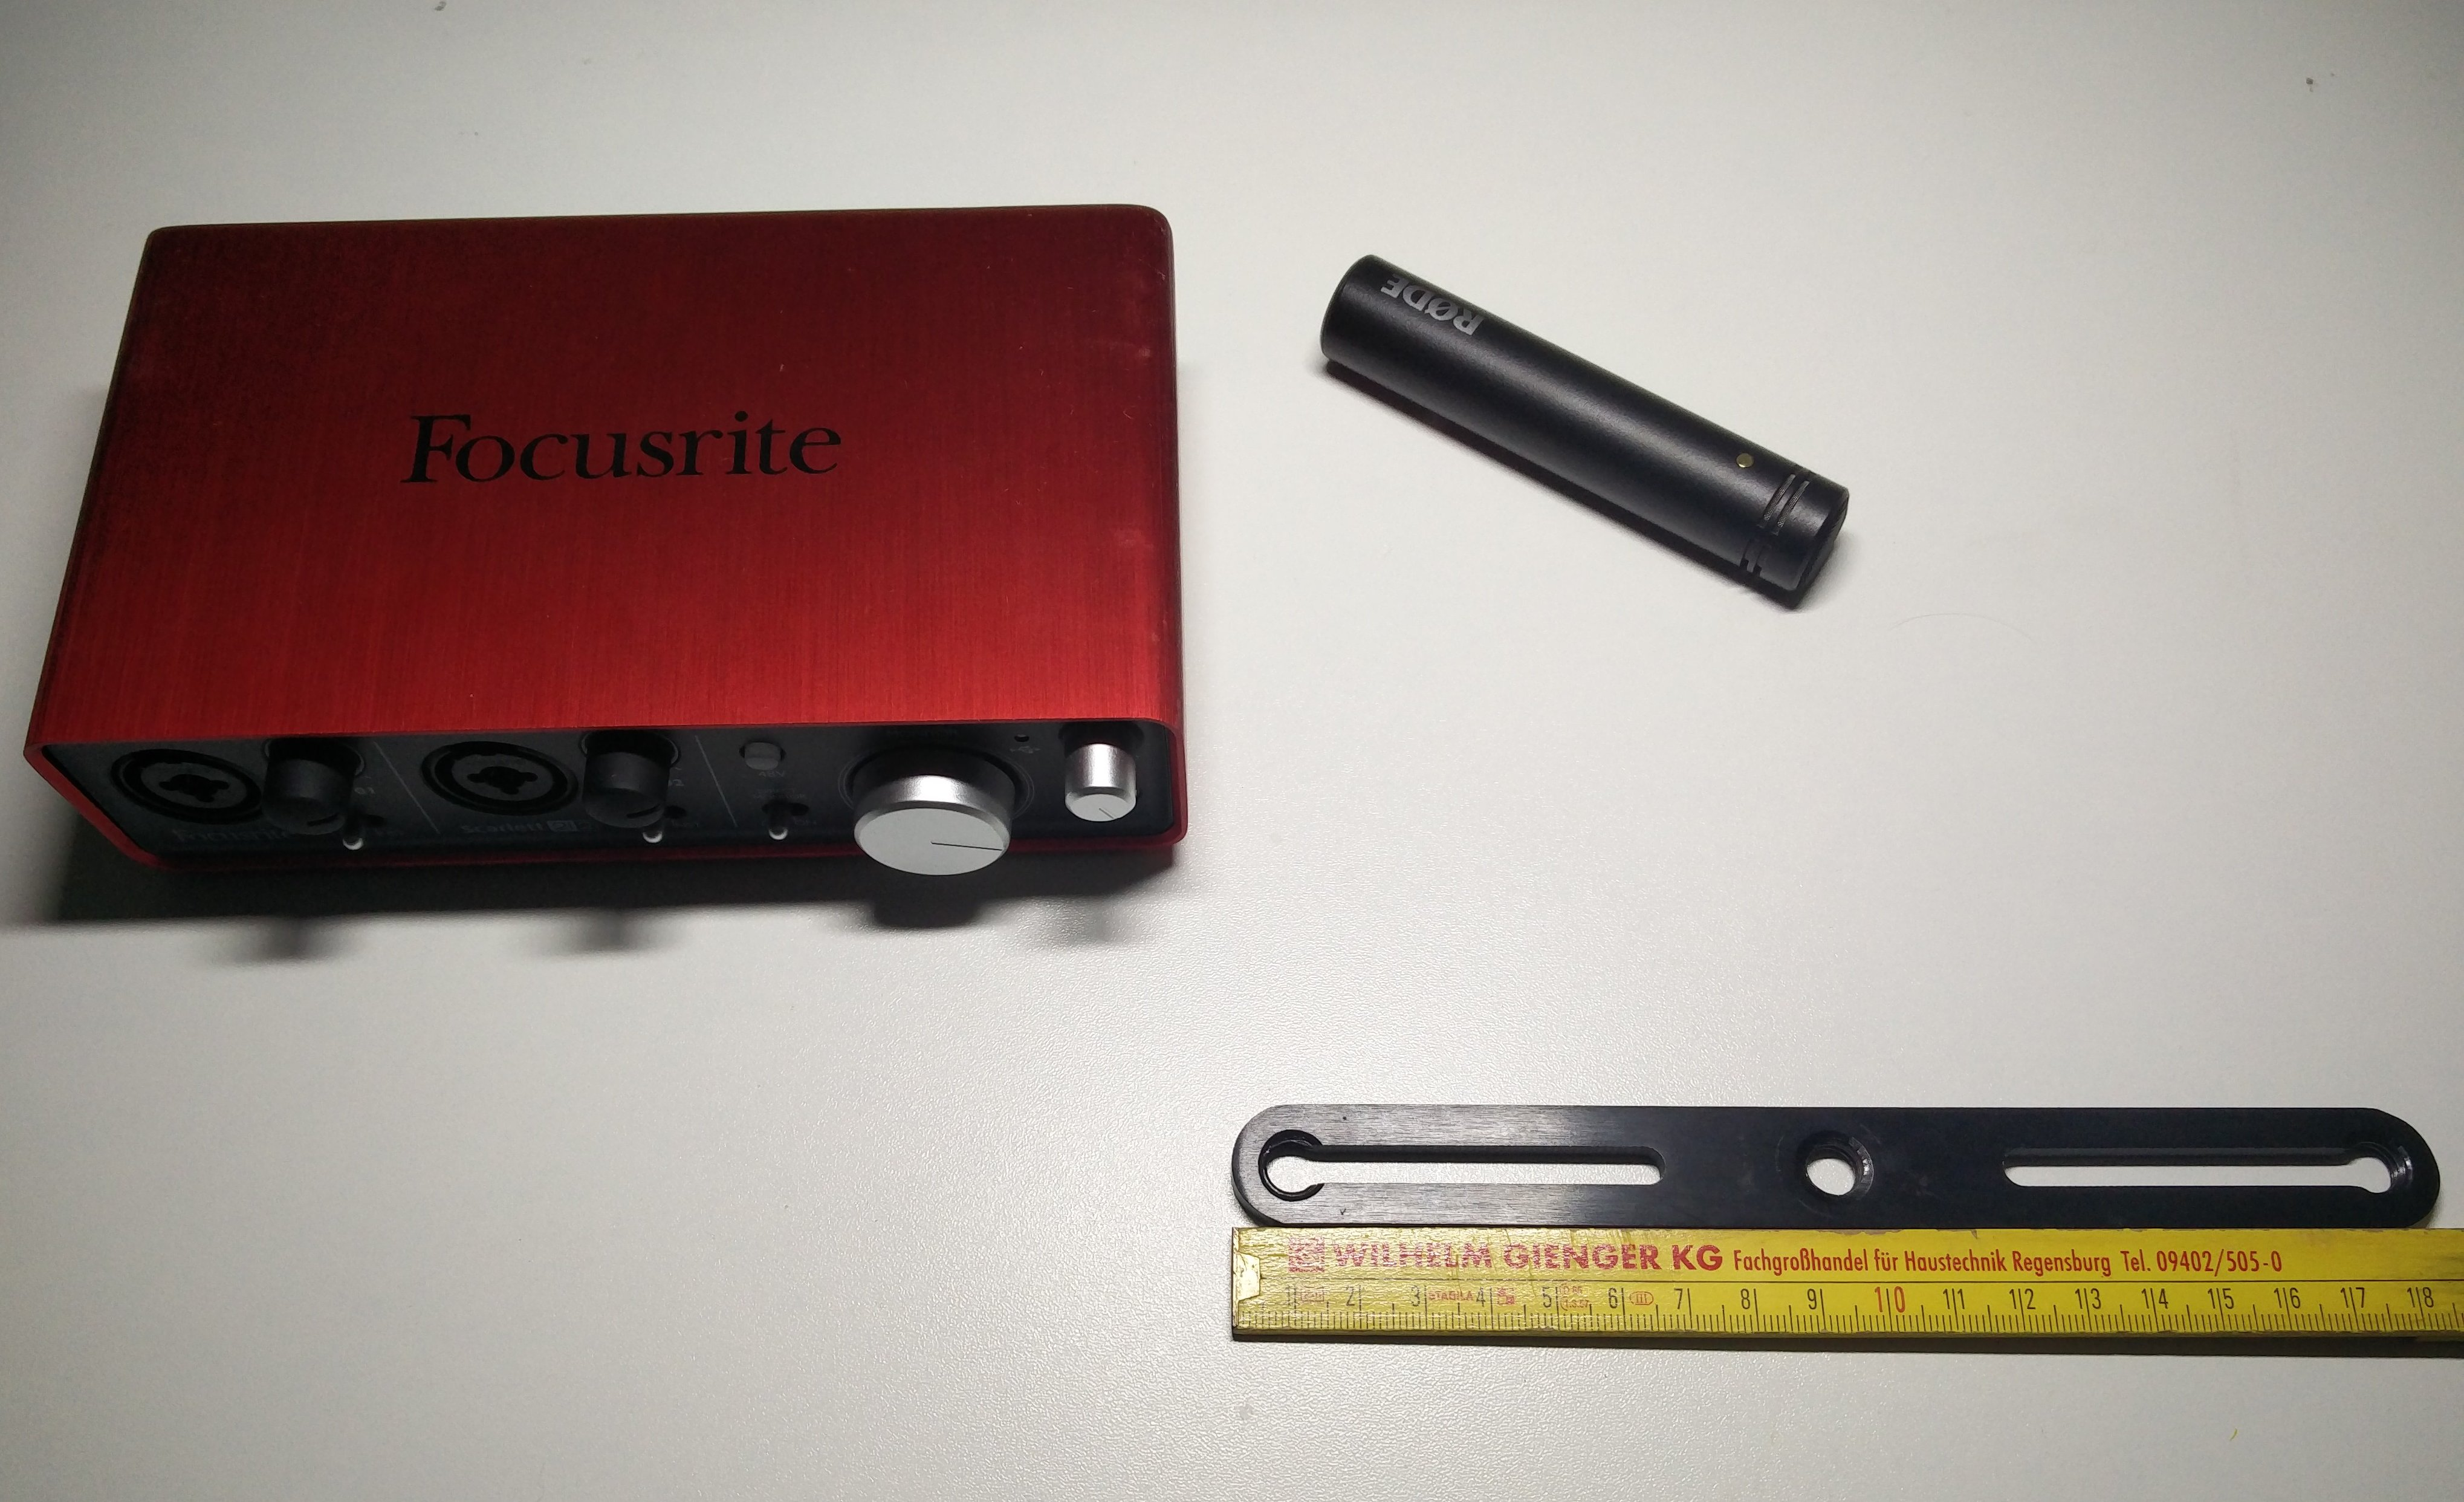
\includegraphics[width=\textwidth]{img/Equipment}
  \caption{Verfügbare Technik}
  \label{material}
\end{figure}
